\documentclass[tikz,multi]{standalone}
\providecommand*{\xMin}{}%
\providecommand*{\xMax}{}%
\providecommand*{\yMin}{}%
\providecommand*{\yMax}{}%
\renewcommand*{\xMin}{0}%
\renewcommand*{\xMax}{4}%
\renewcommand*{\yMin}{0}%
\renewcommand*{\yMax}{4}%
\begin{document}
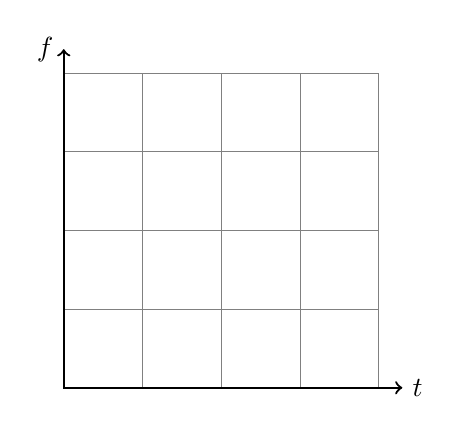
\begin{tikzpicture}
  \foreach \i in {\xMin,...,\xMax} {
    \draw [very thin,gray] (\i,\yMin) -- (\i,\yMax)  node [below] at (\i,\yMin){};
  }
    \draw [very thin,gray] (\xMax,\yMin) -- (\xMax,\yMax)  node [below] at (\xMax,\yMin){};
  \foreach \i in {\yMin,...,\yMax} {
      \draw [very thin,gray] (\xMin,\i) -- (\xMax,\i) node [left] at (\xMin,\i) {};
  }
  \draw [<->,thick] (\yMin,\yMax + 0.3) node (yaxis) [left] {$f$}
    |- (\xMax + 0.3,\xMin) node (xaxis) [right] {$t$};
\end{tikzpicture}
\end{document}
